\subsection{Handhabung der Lizenzen}
\label{sec:handhabung}
\subsectionframe

\begin{frame}{Rechte am Code}
	\begin{itemize}
		\item Eventuell hat man durch Vertrag die Rechte abgetreten
		\begin{itemize}
			\item Anstellungsvertrag
			\item Auftrag
			\item Contributor License Agreement
		\end{itemize}
		\item Rechteinhaber darf mit Code machen was er will
		\begin{itemize}
			\item Mehrfachlizenzierung
			\item verschiedene FLOSS Lizenzen
			\item proprietäre Verwendung
		\end{itemize}
	\end{itemize}
\end{frame}

\begin{frame}{Verwendung mit proprietären Code}
	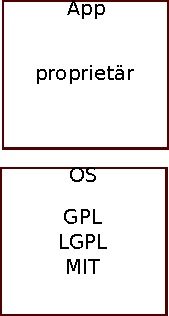
\includegraphics[width=0.2\textwidth]{res/propritary-on-os.pdf}
	\hfill
	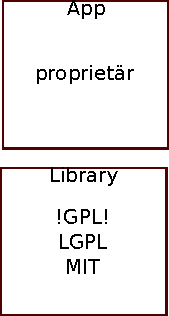
\includegraphics[width=0.2\textwidth]{res/propritary-dynamic-linking.pdf}
	\hfill
	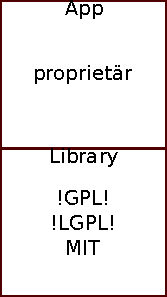
\includegraphics[width=0.2\textwidth]{res/propritary-static-linking.pdf}
	\hfill
	
\includegraphics[width=0.2\textwidth]{res/propritary-use-code.pdf}
	\\
	\todo{schönere Bilder}
	
\includegraphics[width=3em]{res/open-handcuffs.pdf}
	
\includegraphics[width=3em]{res/gnu-head.pdf}
\end{frame}
\note
{
	\begin{itemize}
		\item proprietäre Applikation auf freiem OS (z.B. Debian GNU/Linux) kein Problem
		\item Verwenden in proprietärem Code: nur nachgiebige Lizenzen (MIT)
		\item Linken nur gegen Libraries mit nachgiebige Lizenzen oder LGPL
		\item Code unter Copyleft darf nicht in proprietärer Applikation verwendet werden\footnote{ausser wenn ausschliesslich intern gebraucht, dann ist es Freie Software}
		\item Open Handcuffs: CC-0 by qubodup https://openclipart.org/detail/171929/open-handcuffs
	\end{itemize}
}

\begin{frame}{Verwendung von Code unter Copyleft Lizenz}
	\begin{itemize}
		\item Lizenz Kompatibilität beachten
		\item Patches unter gleicher Lizenz
		\item Contributions schwierig wenn Dual-Lizenziert
	\end{itemize}
\end{frame}

\begin{frame}{Auswahl einer Lizenz}
	\begin{itemize}
		\item Was will man schützen?
		\item Was will man erlauben?
		\item Was will man verhindern? (Gewissen Einsatz verhindern?)
		\item Webseite: \url{http://choosealicense.com/}
	\end{itemize}
	\todo{verschiedene Szenarien auflisten, Beispiele}\\
	MIT \\
	
\includegraphics[width=2cm]{res/gpl-v3-logo.pdf} \\
	
\includegraphics[width=2cm]{res/cc-zero.pdf}
\end{frame}

\begin{frame}{Deklaration der Lizenz}
	\only<beamer:0|handout:1>
	{
	\begin{itemize}
		\item im Projekt (COPYING)
		\item in den Files (SPDX)
		\item in dem Binary (Inkscape)
		\item Keine Lizenz: Code darf nicht benutzt werden
	\end{itemize}
	}
	\begin{center}
		\only<2|handout:2>
		{
			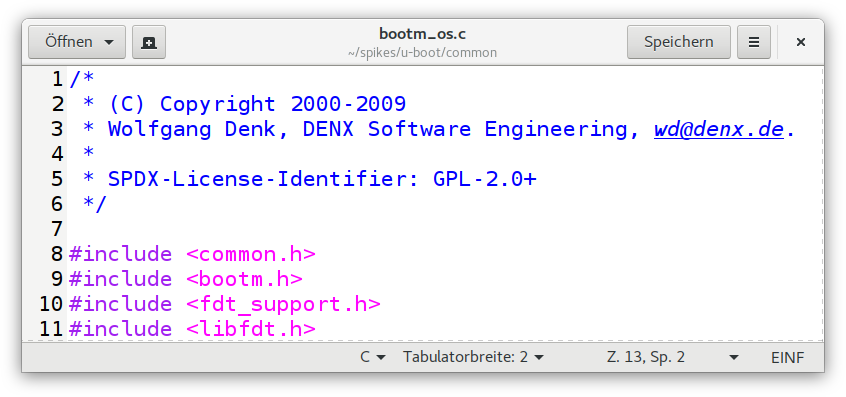
\includegraphics[width=\textwidth]{res/lizenz-source.png}
		}
		\only<3|handout:3>
		{
			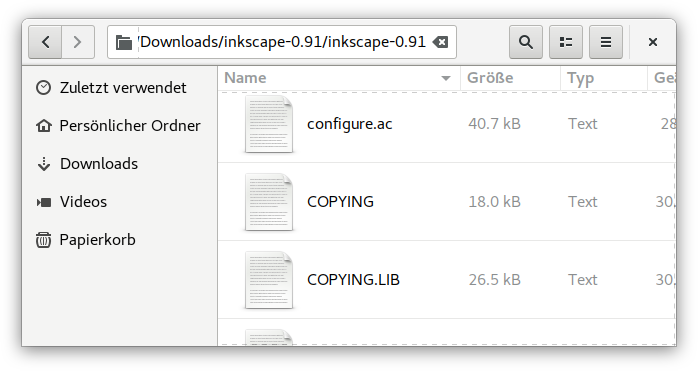
\includegraphics[width=\textwidth]{res/lizenz-file.png}
		}
		\only<4|handout:4>
		{
			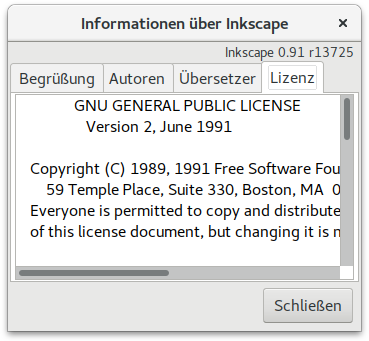
\includegraphics[height=6cm]{res/lizenz-binary.png}
		}
	\end{center}
\end{frame}
\note
{
	\begin{itemize}
		\item im Projekt (COPYING)
		\item in den Files (SPDX)
		\item in dem Binary (Inkscape)
		\item Keine Lizenz: Code darf nicht benutzt werden
	\end{itemize}
}

\begin{frame}{Veröffentlichen der Sourcen}
	\begin{itemize}
		\item öffentliches Repository
		\item Download
		\item Auf Anfrage
	\end{itemize}
\end{frame}

\begin{frame}{Verteidigung des eigenen Codes}
	\begin{itemize}
		\item Dialog suchen
		\item gpl-violations.org \url{https://en.wikipedia.org/wiki/Gpl-violations.org}
		\begin{itemize}
			\item Verschiedene Erfolge, dadurch Gültigkeit der GPL Bewiesen
		\end{itemize}
	\end{itemize}
\end{frame}

\begin{frame}{Best Practises in der FLOSS Community}
	\begin{itemize}
		\item release early
		\item release often
		\item offener Entwicklungsprozess
		\item einfach Kontaktierbar
		\item nett sein
	\end{itemize}
\end{frame}
